\documentclass[aspectratio=169, 10pt]{beamer} % widescreen ratio
% \documentclass[10pt]{beamer} % standard ratio
% background should be changed accordingly
\usepackage[english]{babel}
\usepackage[utf8]{inputenc}
\usepackage{tikz}
\usepackage{graphicx}
\usepackage{helvet} %to use Arial-like font
\usepackage{silence}

\mode<presentation>{
  \usetheme{default}      % or try Darmstadt, Madrid, Warsaw, ...
  \usecolortheme{default} % or try albatross, beaver, crane, ...
  %\usefonttheme{default}  % or try serif, structurebold, ...
  \setbeamertemplate{navigation symbols}{}
  \setbeamertemplate{caption}[numbered]
} 

\setbeamertemplate{background}{
    
\includegraphics[width=\paperwidth,height=\paperheight]{backgroundwidescreen.pdf}
    %
\includegraphics[width=\paperwidth,height=\paperheight]{backgroundstandard.pdf}
}

\setbeamertemplate{headline}{ % to leave some space for the UCI headline
    \vspace{1.4cm} % change depending on font size
}

\setbeamertemplate{footline}{
    \leavevmode%
    \hbox{%
    \begin{beamercolorbox}[wd=.333333\paperwidth,ht=2.25ex,dp=1ex,center]{author in head/foot}%
        \usebeamerfont{title in head/foot}\insertshortauthor
    \end{beamercolorbox}%
    \begin{beamercolorbox}[wd=.333333\paperwidth,ht=2.25ex,dp=1ex,center]{title in head/foot}%
        \usebeamerfont{title in head/foot}\insertshortinstitute
    \end{beamercolorbox}%
    \begin{beamercolorbox}[wd=.333333\paperwidth,ht=2.25ex,dp=1ex,right]{date in head/foot}%
        \usebeamerfont{date in head/foot}\insertshortdate{}\hspace*{2em}
        \insertframenumber{} / \inserttotalframenumber\hspace*{2ex} 
    \end{beamercolorbox}}%
    \vskip0pt%
}
\makeatother
\WarningFilter{latex}{\include should only be }
% For other needed packages
% Put your own preamble here, these might be of use

\usepackage{amsmath, float, graphicx, listings, alltt, multicol, hyperref, amssymb, subcaption}
\usepackage[ruled,vlined]{algorithm2e}

\usepackage{tikz} %for block diagram
\usetikzlibrary{shapes,arrows,positioning}
\tikzstyle{point}=[coordinate]
\tikzstyle{block} = [draw, fill=blue!10, rectangle, minimum height=3em, minimum width=6em, node distance=1cm]
\tikzstyle{prod} = [draw, fill=blue!10, circle, node distance=2cm]
\tikzstyle{pinstyle} = [pin edge={to-,thin,black}]
\tikzset{%
  sbStyleBloc/.append style = {align = center}}

% For outline every section
% \AtBeginSection[]
% {
%     \begin{frame}
%         \frametitle{Outline}
%         \tableofcontents[currentsection]
%     \end{frame}
% }

\newcommand{\R}{\mathbb{R}}
\DeclareMathOperator{\Tr}{Tr}

\title[Beamer template]{Deep Neural Networks}
\subtitle{For the UCI Samueli School of Engineering}
\author{Saketh Karumuri}
\institute{UCI Samueli School of Engineering}
\date{May 6, 2025}

\begin{document}

\begin{frame}[noframenumbering, plain]
    \titlepage
    %thank sponsrs here?
\end{frame}

    \begin{frame}
        \frametitle{Outline}
        \tableofcontents
    \end{frame}
\section{What Are Deep Neural Networks?}

% Should give context and also a why should we care
\begin{frame}{ Mr.Zip Learns to Read}
    \begin{figure}
            \centering
    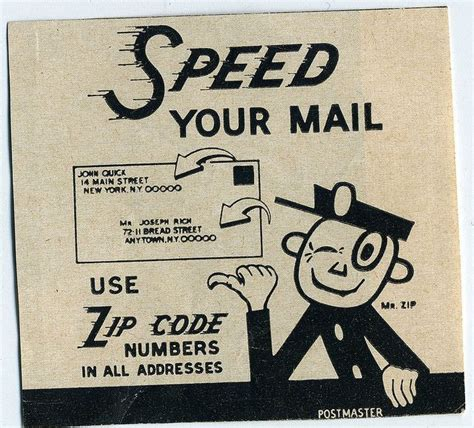
\includegraphics[width=0.2\textwidth]{mrzip.jpg}
    \end{figure}
    % TODO: Image of ZipPostalWorker
    % Image of number from MNIST Dataset?
  You work for the post office during the dawn of character recognition. \par How can you make an algorithm that can go from an image to a zip code?\par 
\end{frame}\begin{frame}{ Mr.Zip Learns to Read}
    \begin{figure}
            \centering
    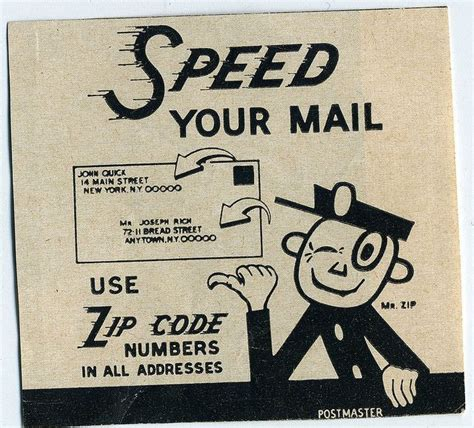
\includegraphics[width=0.2\textwidth]{mrzip.jpg}
    \end{figure}
    % TODO: Image of ZipPostalWorker
    % Image of number from MNIST Dataset?
  Thankfully, you paid enough attention in bio to learn that our neurons can represent anything we can think of (literally) \par
  Lets make a "brain" out of these neurons. Now we can "teach" it by showing it what numbers look like and seeing how the neurons are activated. \par
  We've just come up with neural networks!
\end{frame}

\begin{frame}{What Are Neural Networks?}
    \begin{figure}
            \centering
            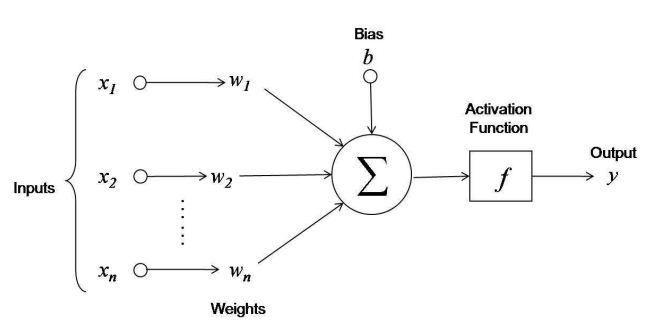
\includegraphics[width=0.3\textwidth]{./NNDetailed.jpg}
    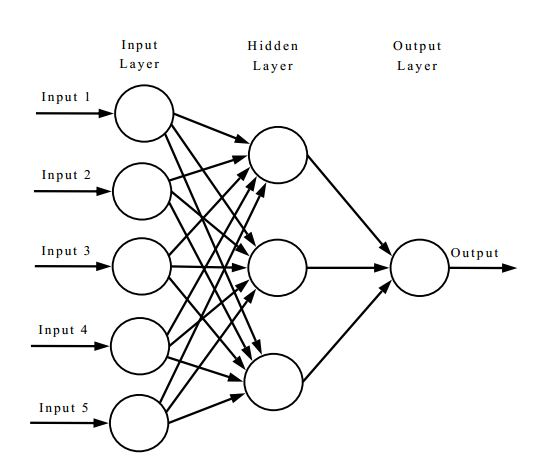
\includegraphics[width=0.3\textwidth]{./ann_overview.jpg}
    \end{figure}
    % TODO: Image of Neural Networks (show one with many layers) and show one with symbols for addtions and stuff
    Neural Networks \begin{itemize}
        \item inspired by biological neurons
        \item have input stimulus, activation function and output can be used as the networks output or as the input of other neuron(s)
        \item built up of 1 input layer, a number of hidden layers, and 1 output layer.
    \end{itemize}
  % Model neurons by having an "activation function" that responds to an input stimulus
  % Training is setting the weights and biases for this neuron.
  % Training is in essence, figuring out which neurons should connect to each other and how much influence they should have over eachother to represent the function we're approximating.
\end{frame}

\begin{frame}{Neural Networks are function approximators!}
     \begin{figure}
            \centering
    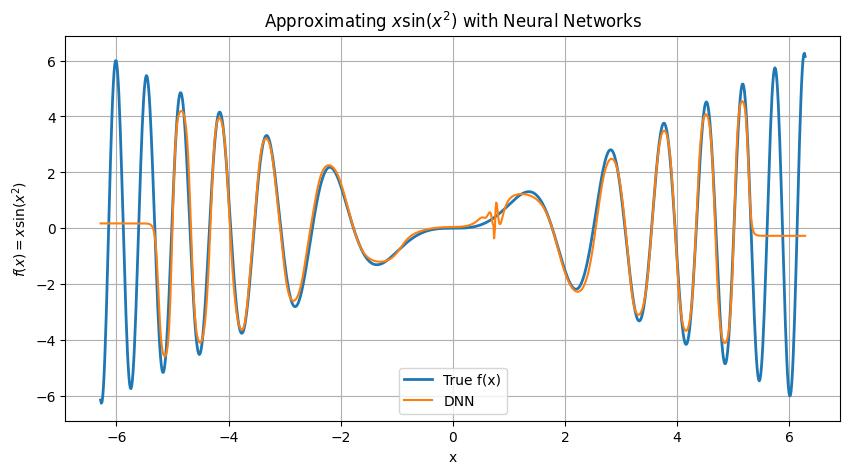
\includegraphics[width=0.5\textwidth]{./just1ExampleEstrimateion.png}
    \end{figure}   % Show image of function being approximated!

  Training is the process of finding which neurons need to be connected to eachother and what level of stimulus they activate at to best approximate the desired function.
  Neural Networks with one arbitrarily sized hidden layer  don't need any more than one hidden layer to represent any function.
%(with non-linear activation functions)
\end{frame}

\begin{frame}{Why Approxmiate Functions}
    %TODO: Example images of NN Applications
  Not all functions we work with can be easily represented analytically so for us to do useful things in reasonable time frames we need to represent them. Some examples of functions that would be nice to have analytic solutions to are: \begin{itemize}
      \item What will the weather tomorrow be as a function of climate data gathered today
    \item What number is this image's pixel data trying to represent?
    \item How should I steer to maximize the likely hood that the car does not crash?
    \end{itemize}
\begin{figure}
            \centering
    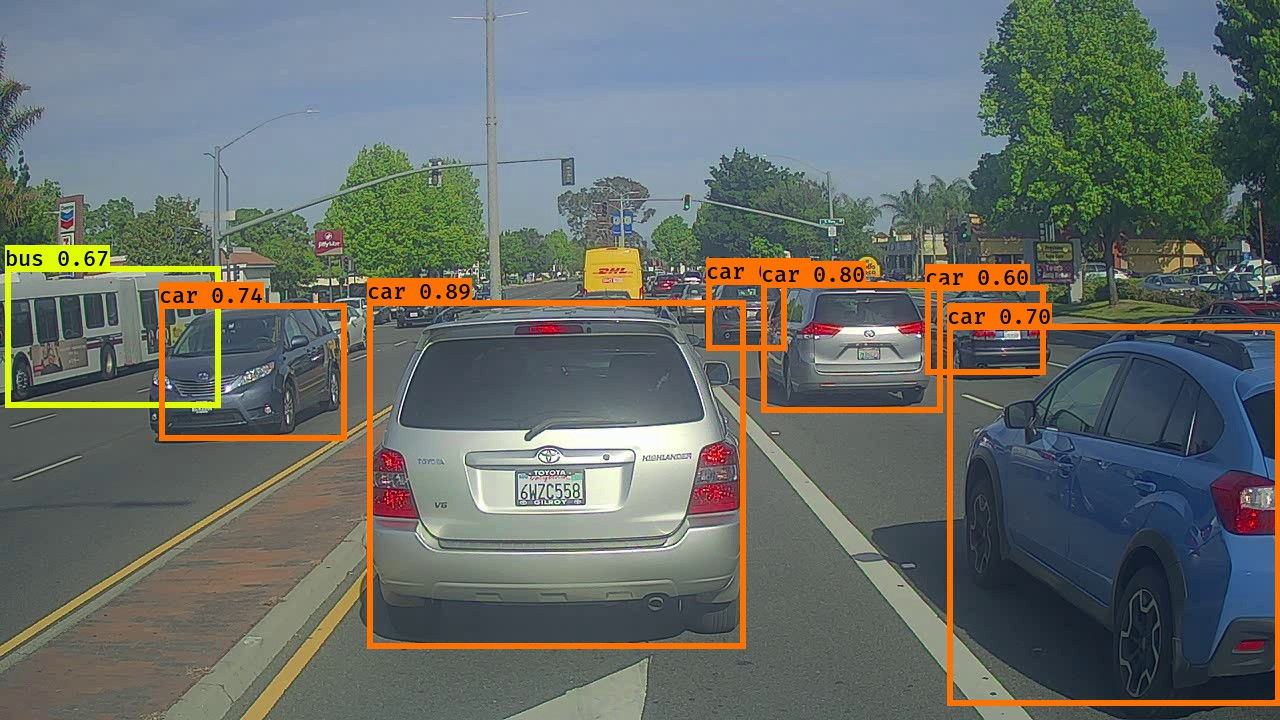
\includegraphics[width=0.4\textwidth]{./yolo_Ex.jpg}
    \end{figure}\end{frame}
     
\begin{frame} {What Are Deep Neural Networks (DNNs)?}

\end{frame}\begin{frame} {What Are Deep Neural Networks (DNNs)}
  % TODO: Image of shallow vs. Deep Neural Network Deep Neural Networks are what we call Neural Networks when they have multiple hidden layers.

    Deep Neural Networks have more than one Hidden Layer.
  % Do you need to say why this kind of approximation is strong
  % Figure of single, multi layer perceptrons
  % Math of the weights, inputs activation functions etc.
  % Mention how backpropogation makes optimization easier
  % Training is picking the right weights
  % Single layer stuff was 90s 2000s we had strngth of multi layer
  % static Univerfal Function approximator (can make a lot of problems functions)
  % Technically Lipschitz Continuous?
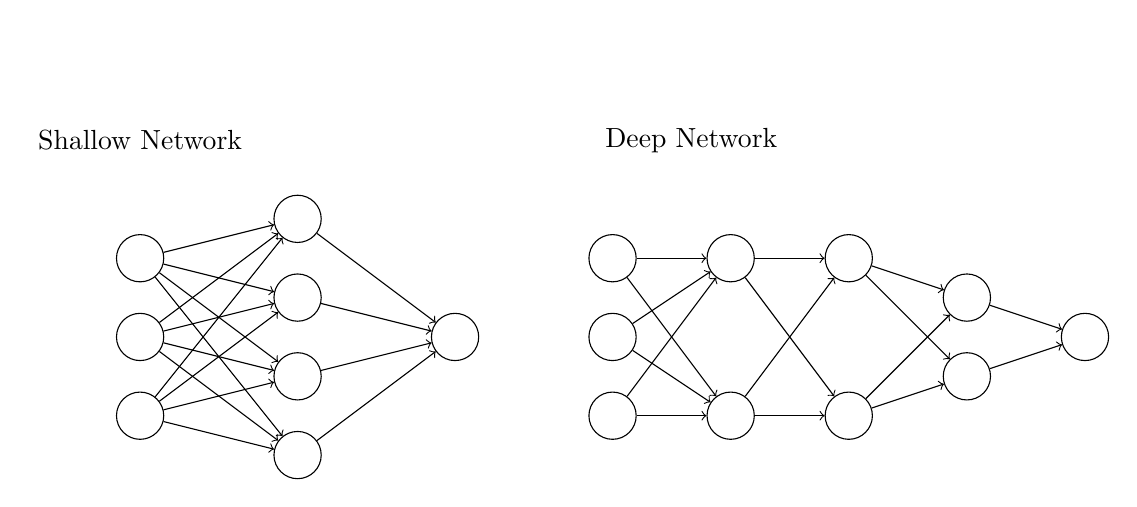
\begin{tikzpicture}[node distance=0.8cm and 0.8cm, every node/.style={circle, draw, minimum size=6mm}, scale=1]

% Shallow Network
\node[draw=none] at (0, 2.5) {Shallow Network};
\node (i1) at (0, 1) {};
\node (i2) at (0, 0) {};
\node (i3) at (0, -1) {};

\node (h1) at (2, 1.5) {};
\node (h2) at (2, 0.5) {};
\node (h3) at (2, -0.5) {};
\node (h4) at (2, -1.5) {};

\node (o) at (4, 0) {};

\foreach \i in {i1,i2,i3}
    \foreach \j in {h1,h2,h3,h4}
        \draw[->] (\i) -- (\j);

\foreach \j in {h1,h2,h3,h4}
    \draw[->] (\j) -- (o);

% Deep Network
\node[draw=none] at (7, 2.5) {Deep Network};
\node (di1) at (6, 1) {};
\node (di2) at (6, 0) {};
\node (di3) at (6, -1) {};

\node (dh1) at (7.5, 1) {};
\node (dh2) at (7.5, -1) {};

\node (dh3) at (9, 1) {};
\node (dh4) at (9, -1) {};

\node (dh5) at (10.5, 0.5) {};
\node (dh6) at (10.5, -0.5) {};

\node (do) at (12, 0) {};

\foreach \i in {di1,di2,di3}
    \foreach \j in {dh1,dh2}
        \draw[->] (\i) -- (\j);

\foreach \i in {dh1,dh2}
    \foreach \j in {dh3,dh4}
        \draw[->] (\i) -- (\j);

\foreach \i in {dh3,dh4}
    \foreach \j in {dh5,dh6}
        \draw[->] (\i) -- (\j);

\foreach \j in {dh5,dh6}
    \draw[->] (\j) -- (do);

\end{tikzpicture}
\end{frame}

\begin{frame} {Why Do we Need Depth?}
  Depth generally improves performance.
  % TODO: Image of NN Loss Graph with explanation
     \begin{figure}
            \centering
    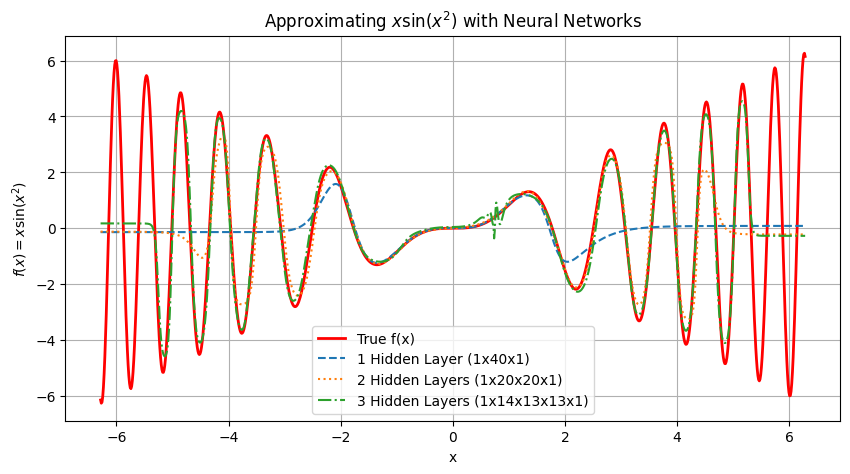
\includegraphics[width=0.45\textwidth]{./ExampleOfFunctionEstimation.png}
    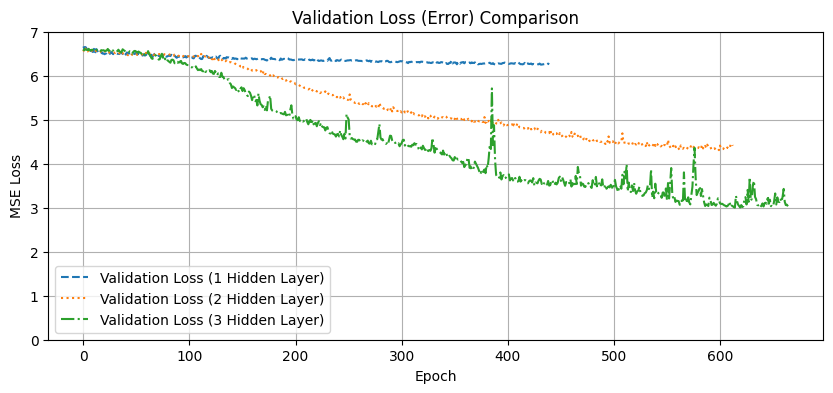
\includegraphics[width=0.45\textwidth]{./lossBetweenNHiddenLayers.png}
    \end{figure}   % Show image of function being approximated!
  
\end{frame}

\begin{frame}{But \textit{Why} Do we Need Depth?}
    For a network with \begin{itemize}
        \item $m$ - inputs
        \item $L$ - layers
        \item $n>m$ neurons 
    \end{itemize}
    With ReLU activation, this network can represent a piecewise linear function with a lower bound on the number of segments $$\Omega\left(\left(\frac{n}{m}\right)^{L-1}n^m\right)$$
    \tiny https://arxiv.org/abs/1312.6098 \par
    http://papers.nips.cc/paper/5422-on-the-number-of-linear-regions-of-deep-neural-networks
\end{frame}

\begin{frame}{We don't understand how these work}
    % this is honestly why I'm interested in this
    There are so many parameters that it being able to fit to any training data makes sense. But doesn't make sense is how it's able to actually learn when given real data if it's overfitting to random noise?
    \par
    %\tiny     https://dl.acm.org/doi/10.1145/3446776

\end{frame}

\section{How Do You Solve Problems With DNNs}
\begin{frame}
    \huge What does using a DNN to solve a problem look like?
\end{frame}

\begin{frame}{Our Problem}
\end{frame}

\begin{frame}{Our Problem}
    Two robots want to cross a landscape $q$. $q$ is a string of terrain types in the set of terrain types $\mathcal{T}= \{ \tau_1,\tau_2, \dots,\tau_p \}$. We have Terrain resistances for robot $i$: $c_i(t)$ where $t \in \mathcal{T}$
  Our decision variable is $\sigma$ the mode indicator.
\begin{equation*}
  \sigma : \mathcal{T} ^N \to \mathcal{ M }^N
\end{equation*}
\begin{itemize}
    \item $\mu_i$ - mass of robot $i$
    \item $M_i(m)$ - Effective Mass function
    \item where $m$ is the collaborative mode
\end{itemize}
Our effective mass functions are defined as:
\begin{equation}
  M_1(m) = \begin{cases}
    \mu_1 & \text{ if } m=0\\
    \mu_1 + \mu_2 & \text{ if } m=1\\
    0 & \text{ if } m=2
  \end{cases}
  , \hspace{15px}
  M_2(m) = \begin{cases}
    \mu_2 & \text{ if } m=0\\
    0 & \text{ if } m=1\\
    \mu_1 + \mu_2  & \text{ if } m=2
  \end{cases}
\end{equation}
  
\end{frame}
\begin{frame}{Our Problem}
The energy consumed by each robot for a given assignment string is
\begin{equation}
  E_i(\sigma) = \sum_{ k=1 }^N\left[ c_i(q_k) M_i(\sigma_k)+c_{si} \delta( {\sigma_{k-1},\sigma_k} )\right]
\end{equation}
\begin{equation}
  \delta(m_i,m_j) = \begin{cases}
    1 & \text{ if } m_i \neq m_j \\
    0 & \text{otherwise}
  \end{cases}
\end{equation}
Where $\sigma_0=0$,\par
Finally, we want:
%$q_k$ is the $k$th element of the landscape $q$ and $c_{si}$ is the switching cost for the robots to change collaboration modes. 
\begin{equation}
  \min_\sigma \left\|\begin{bmatrix}
    E_1(\sigma)\\E_2(\sigma)
  \end{bmatrix}\right\|_p
\end{equation}
\end{frame}
\begin{frame}{The Traditional Approach\dots}
  Usually we would use something called a Mixed Integer Linear Program which uses decision variables to find the decision variable's values for the minimum (or maximum) value of the function. 
\par
\begin{equation}
    |\sigma| \propto O(|\mathcal{T}|^N)
\end{equation}
    Since the action chosen with mixed integer program is a decision variable, the number of decision variables we have scales with the length of terrain.
\end{frame}

\begin{frame} {Why Use a DNN here?}
  Neural Networks can estimate a function that gives us the optimal assignment. Neural networks scale at a much more reasonable rate as we increase the number of layers (however it remains to be seen how much training time increases as a result of this as well).
  We can effectively design a network to be exactly as big (and computationally expensive) as we want.
\end{frame}

\begin{frame}{Designing our Network}
    Rules of Thumb \begin{itemize}
      \item Generally DNNs use no more than 3 layers \par
      \item Bigger hidden layers than input layers \par
      \item Aside from this it's a lot of experimenting on your specific problem
    \end{itemize}
    \par
    We can use a DNN by \textit{embedding} our inputs to get numerical values to give as inputs to the NN\par
    Similary for our output we need to do the opposite to get the network's estimated solution.
    %
    % To go from letters to inputs we need an "embedding"
    % Whatever embedding is chosen it needs to be able to represent the state of the whole world. I used $n_{terrains}^{l_{window}}$
    % Then use linear activation for last nodes and pick % convince someone that this is worth their time
    %
    % What can attention do for us? Attention could allow for the network to focus on segments of terrain that have more of an impact on the optimal assignment strategy.
\end{frame}
\begin{frame}{Future Work}
    For this neural network estimation to be useful we need to estimate a system with more robots or use a longer terrain to be crossed. \par
    In both cases this causes a big increase in computing the optimal solution: $|\sigma| \propto O(|\mathcal{T}|^N)$
    I have reworked the problem to be something that is a Model Planning Control problem that's solved online. I still want to find at what point it becomes reasonable to use the DNN to approximate the solution.
\end{frame}
\end{document}
